% algorith2e macros:
\SetKwFor{Procedure}{procedure}{is}{end procedure}
\SetKwInOut{Requires}{Requires} % precondition (assumed)
\SetKwInOut{Ensures}{Ensures} % postcondition (guaranteed)
\SetKwInOut{Uses}{Uses} % variables used
\SetKw{DownTo}{downto}
% for nondeterministic choice:
%\SetKwIF{Choose}{ChooseOr}{ChooseLast}{choose}{}{or}{or}{end}
% \SetKwSwitch{Choose}{ChooseCase}{ChooseOther}{choose}{}{when}{}{}
\SetKwFor{WhileChoose}{while}{do choose}{}
\SetKwFor{While}{while}{do}{}
\SetKwFor{ForAny}{for any}{do}{}
\SetKwIF{When}{Unused}{Unused}{when}{}{}{}{}

\newcommand{\nxl}{\textup{\textsf{nxl}}} % number of local cells (COLUMNS) excluding ghosts
\newcommand{\nyl}{\textup{\textsf{nyl}}} % number of local cells (ROWS) excluding ghosts
\newcommand{\tm}{ \text{$t_{max}$} }
\newcommand{\av}{ \mathbf{a} }
\newcommand{\uv}{ \mathbf{u} }
\newcommand{\bv}{ \mathbf{b} }
\newcommand{\pv}{ \mathbf{p} }
\newcommand{\orig} {\mathcal{O}}

\newcommand{\rnt}{ R_{-\theta} }
\newcommand{\rt}{ R_{\theta} }

\newcommand{\la}{\leftarrow} % for assignments
\newcommand{\ra}{\rightarrow} % for assignments

\newcommand{\dx}{\textsf{dx}}
\newcommand{\dy}{\textsf{dy}}

\newcommand{\data}{\textup{\textsf{data}}}
\newcommand{\psendf}{\textit{postSend}}
\newcommand{\precvf}{\textit{postRecv}}
\newcommand{\psend}[2]{\psendf(#1,#2)}
\newcommand{\precv}[2]{\precvf(#1,#2)}
\newcommand{\pid}{\textup{\textsf{pid}}} % my rank


\begin{figure}[t]
  \centering
  \includegraphics[width=0.6\textwidth]{classic_division.eps}
  \caption{4 process decomposition of a 22x16 stencil.  Process labels start in the top left and proceed clockwise.  Local
  variables of state are also illustrated for indexing a 2D array, 0,1,$B_x^1$,etc.}
  \label{fig:basic}
\end{figure}

\section{Motivation And Basic Terminology}\label{sec:problem_statement}

The solutions of partial differential equations (PDEs) are classic problems for parallel
computers and use
what are known as stencil methods.
Figure~\ref{fig:basic} illustrates an example of a {\it stencil}
for a 2D PDE at grid cell $(B_x^1,B_y^1)$ of process 4.
At cell $(B_x^1,B_y^1)$ there is a single blue circle surrounded by 4 circles.
This structure is known as a {\it 5-point stencil} for the 5 blue circles in the image,
and it is derived from the underlying discretization of the PDE being solved.
The grid cell containing the
center circle is the spatially dependent value of the PDE at a given point in
 time.
The cells of the adjacent circles are the
spatial dependencies for the center cell.

\begin{wrapfigure}{r}{0.5\linewidth}
  \centering
  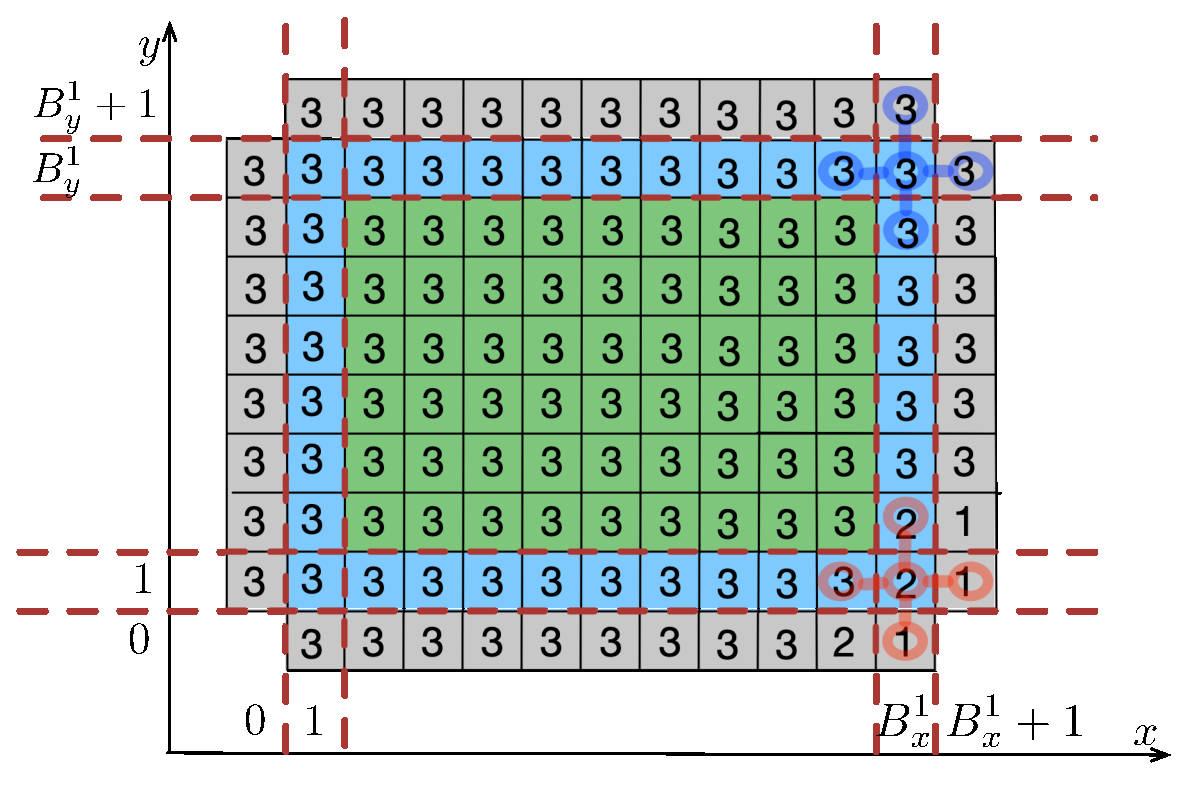
\includegraphics[width=0.5\textwidth]{timeStepDependencies.eps}
  \caption{An illustration of grid cell timestep, and its relationship to
  stencil dependencies.  In cell $(B_x^1,B_y^1)$ dependencies are met, and a
  valid update of the cell can be performed.  In cell $(B_x^1,1)$ the opposite
  is true.  Transparent blue and red circles are overlaid respectively
  for valid and invalid dependencies.}
  \label{fig:timestep}
\end{wrapfigure}

Because these spatial dependencies are functions of time,
whenever a PDE's value is updated once at a grid cell, the dependency
structure changes for that grid cell.
The unit of time taken for a cell update
 is referred to as the {\it timestep} of that cell.
  Figure~\ref{fig:timestep} illustrates the timestep at each cell of process 4
from figure~\ref{fig:basic},
for some arbitrary point during the execution of a stencil method.  It
demonstrates how the spatial dependencies of each cell can change
with time.  The cell
$(B_x^1,B_y^1)$ has a time step of 3, and so do all of its adjacent cells.
When a cell has neighbors above, below, left, and right of it which contain
values computed from the same timestep, we'll say the cell's
dependencies are {\it valid} at a given point in time.  When any one of its
neighbors does not contain a value from the same timestep, then its
depencies are {\it invalid}.  An example of invalid dependencies is given in
cell $(B_x^1,1)$ in figure~\ref{fig:timestep}, where the value of the PDE
is only completed up to the 2nd timestep, and it's neighboring cells
contain values from different timesteps.

This dependency structure has an impact on the performance of any
parallelization strategy for the stencil method.
Parallelizing a large 2D stencil using a SIMD
strategy starts with the definition of a global area over which
computation is required, followed by a subdivision of that area
into 2D grids for each
processing unit to manage.  Figure~\ref{fig:basic} illustrates the general principle for 4 processing units,
each with separate
11x8 grid portions of the total 22x16 global grid size.  While there are indeed 13x10 grid cells for each
process subdivision illustrated, the gray cells for each process are in fact redundant, and they
hold information which come from the adjacent blue cells held by neighbor processes hence the term {\it ghost} cells
indicated in the diagram key.  To make the example explicit, cells $(1,1) - (B_x^1,1)$ of process 1 need to be
reflected in cells $(1,B_y^1+1) - (B_x^1, B_y^1+1)$ on process 4 in order for it to compute cells
$(1,B_y^1) - (B_x^1, B_y^1)$.
  This interprocess dependency is a direct result of the 5 point stencil described above.
  Because of this dependency structure, each process' illustated blue region
({\it border region}) must have up to date records in their ghost regions from the corresponding
 blue region of the nearest process on each side.

This dependency structure between processes is known as a {\it nearest neighbor} dependency structure, and divides
each process' local grid into 9 distinct {\it regions} depending on where they are positioned relative
 to ghost cells which
must be received from neighbor processes.  Continuing to use process 4
in figure~\ref{fig:basic} as an example, the
regions are the green
shaded {\it interior region}, and then 8 blue shaded border regions.  The interior region depends only on border
regions, and is therefore relatively independent of neighbor processes (that independence will be later quantified).
The border regions have 2 types of dependence.  The first type depends on only one neighbor process.  This is
given by cell ranges on the 4 sides of the 2D grid: $(2,1) - (B_x^1 - 1, 1)$, $(1,2) - (1,B_y^1 - 1)$,
$(2,B_y^1) - (B_x^1 - 1, B_y^1)$, and $(B_x^1,2) - (B_x^1,B_y^1 - 1)$.  In these ranges only the gray ghost cells
 received from a single process are
needed to successfully compute grid cells at each point.  The other type of
border region depends on 2 processes and exists solely
in the corners of the 2D grid at cells: $(1,1)$, $(1,B_y^1)$, $(B_x^1,B_y^1)$,
and $(B_x^1,1)$.

Given the 9 static regions described, if a process wishes to execute a complete
timestep for each cell in its grid, it must synchronize the pace of its timesteps
with each neighbor process .
If synchronizations are expensive this creates a performance bottleneck, and
it becomes beneficial
to develop strategies to relax these synchronization requirements.
In order to do so while maintaining
valid stencil dependencies reqires relaxing the boundaries of the 9 classically
static regions of a 2D stencil
on each process.  In the next section we'll describe how this is done, before
developing a concise approach for performing region updates only when
the region contains valid dependencies for each cell.

% TODO: Add diagram from topc paper of the time dimension of dependencies, and put them somewhere
% (or a 2D timelapse of halos)
ْ
% The final dimension of the dependency structure is time, and can be quantified per grid cell, per process region,
% or per global stencil computation.  We say that a grid cell completes its {\it timestep} when it updates
% the physical property being modeled in the grid cell using the the neighbor cells it depends (i.e. top right
% of process 4 in figure~\ref{fig:basic}).

\section{State Variables For Region Decomposition}\label{sec:state}

\begin{figure}[t]
  \centering
  \begin{subfigure}[t]{.5\textwidth}
    \centering
    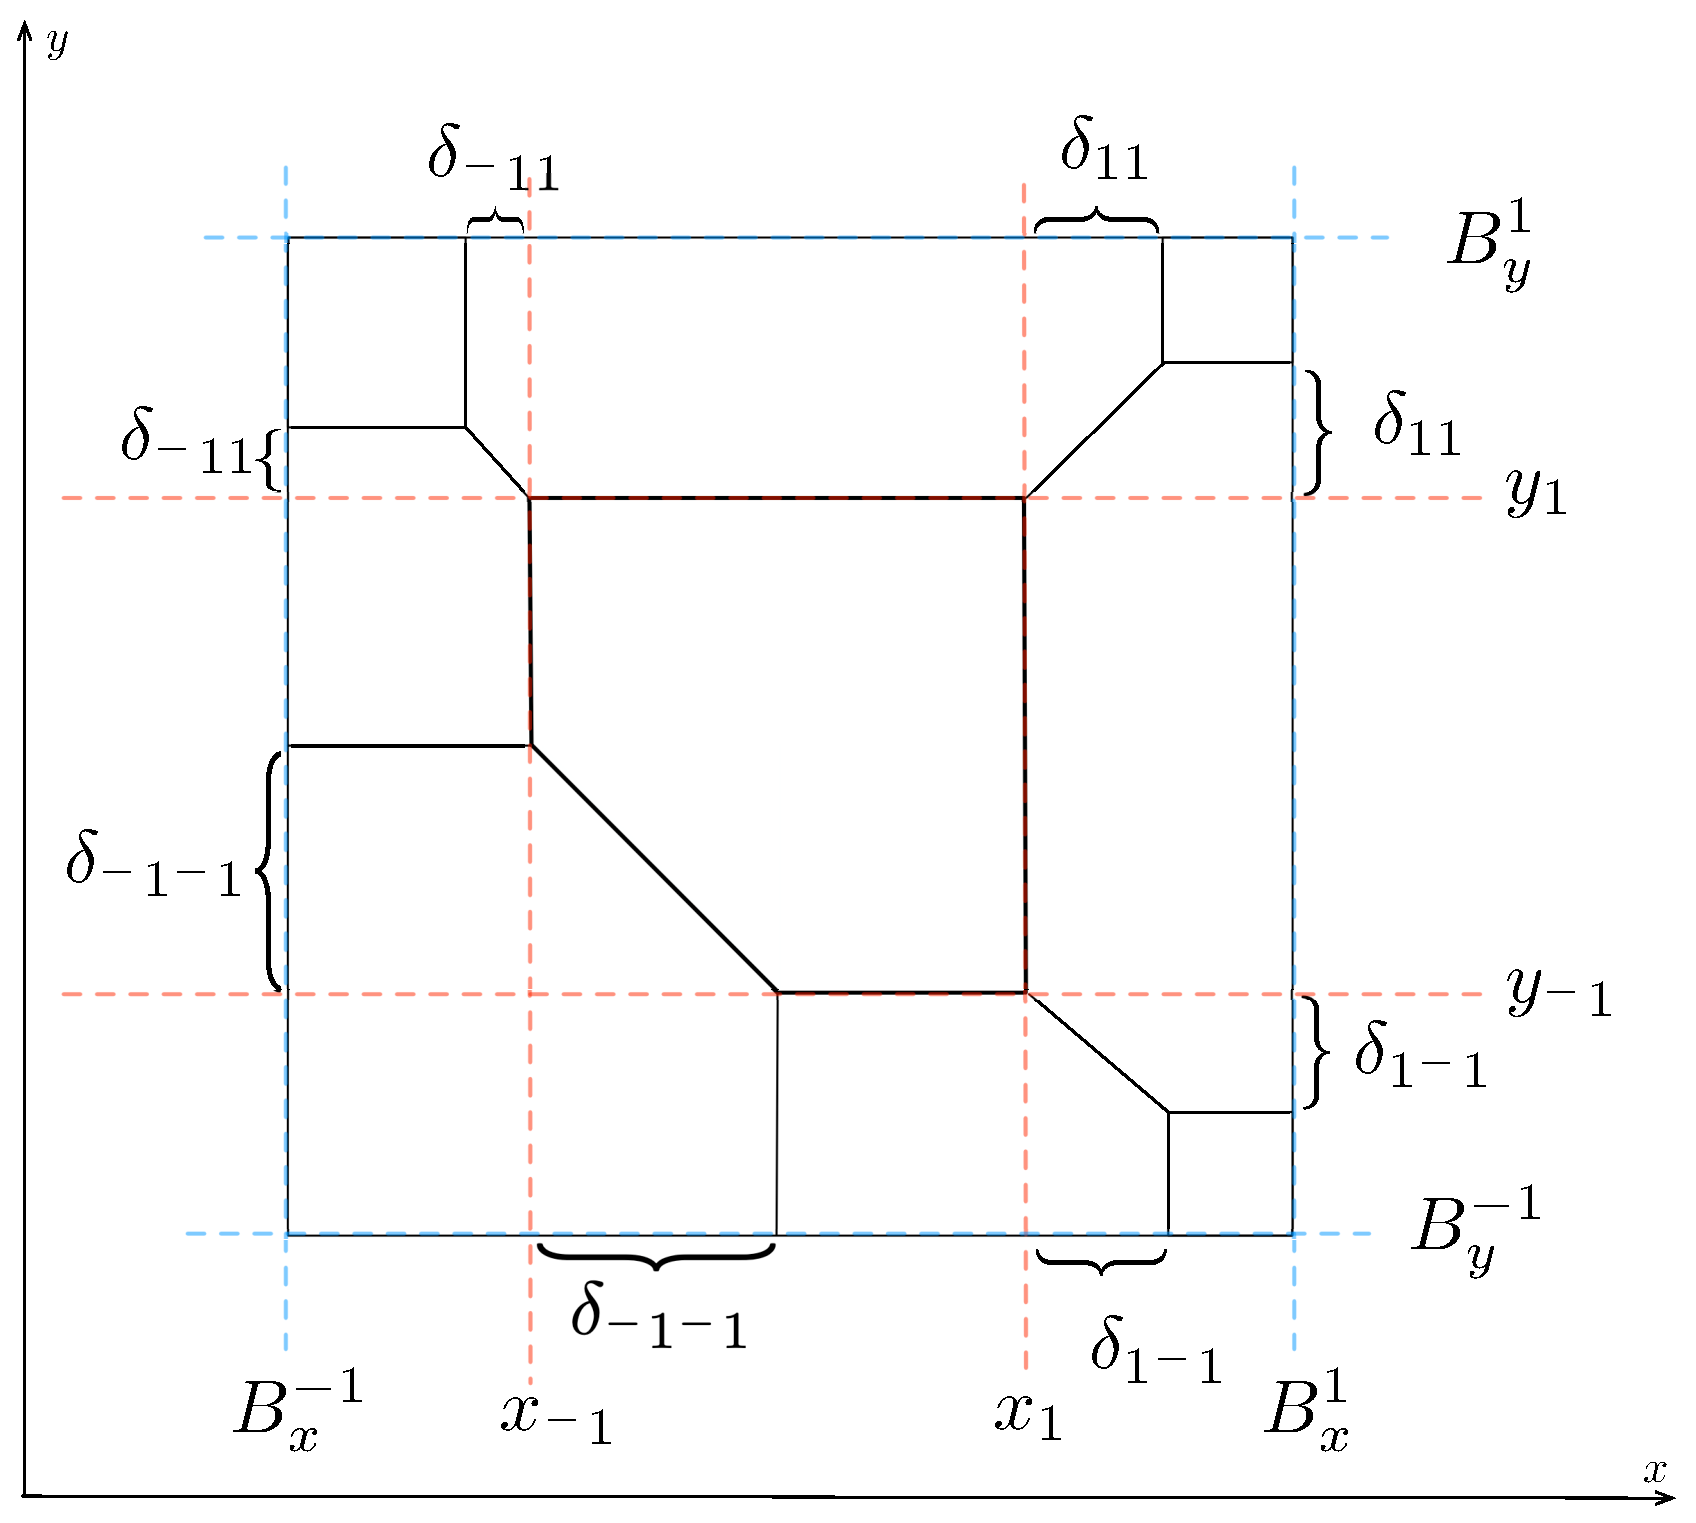
\includegraphics[width=.8\textwidth]{variable_divisions.eps}
    \caption{State maintained for the purpose of extrapolating all area boundaries}
    \label{fig:state_labels}
  \end{subfigure}
  ~
  \begin{subfigure}[t]{.4\textwidth}
    \centering
    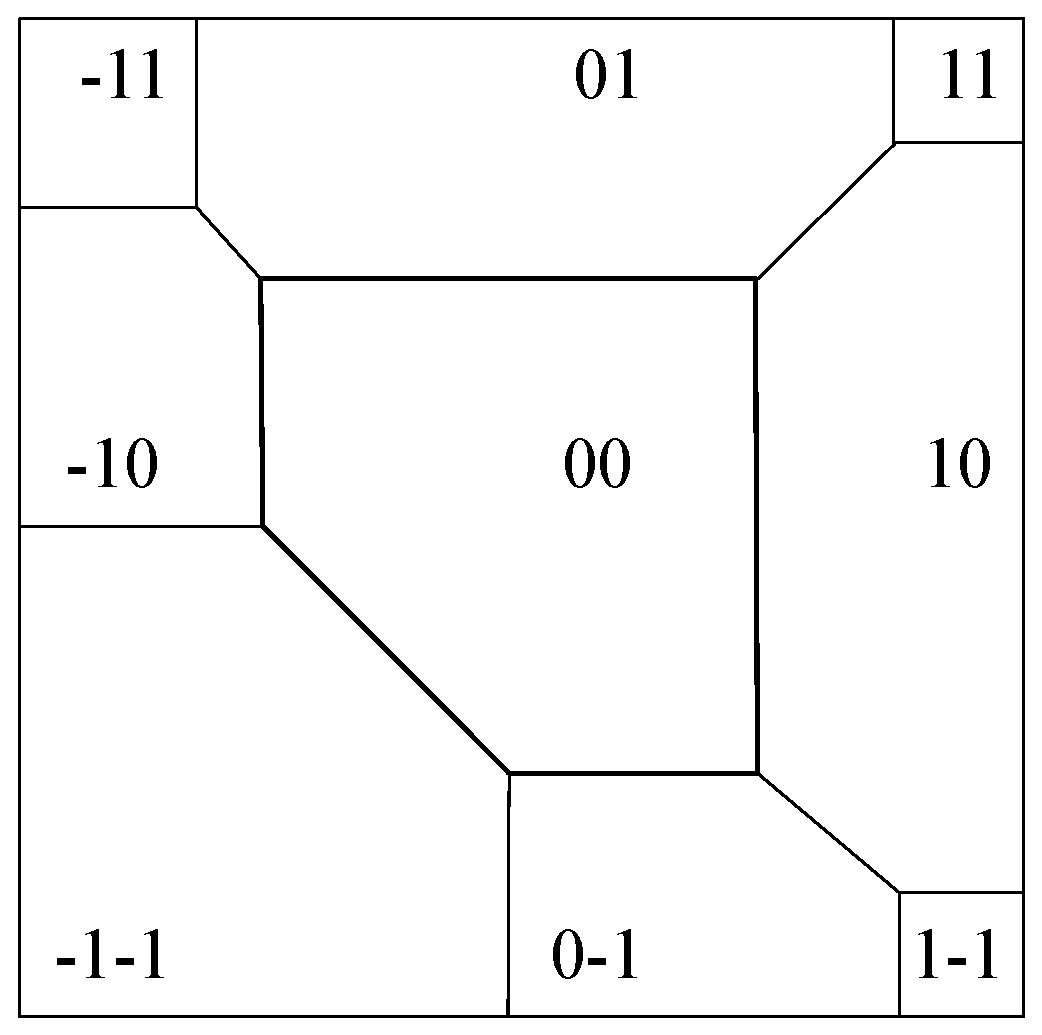
\includegraphics[width=\textwidth]{prior_art_relable.eps}
    \caption{Region labels, each given by 2 digits in the form $a_xa_y$ throughout the rest of the document.
    $a_xa_y$ additionally provides a shorthand for the vector $[a_x\;\;\; a_y]^T$, and we therefore refer to
    these region labels as region vectors, or area vectors throughout the document.}\label{fig:region_vectors}
    \end{subfigure}
  %\includegraphics[width=0.4\textwidth]{region_map.pdf}
  \caption{(\ref{fig:state_labels}) An illustration of state labels that allow each of the 9 regions to relax their
  boundaries.  (\ref{fig:region_vectors}) Shorthand labels for each region, and for corresponding area vectors.}
  \label{fig:local_decomposition}
\end{figure}

Figure~\ref{fig:region_vectors} illustrates a more concise labeling of
each of the 9 regions described above, whose boundaries have been relaxed to arbitrary positions.
  Figure~\ref{fig:state_labels} illustrates the minimal set of variables needed to relax region boundaries
for a single process, and delimits the regions they collectively form.
With these dynamic variables of state, each process has enough information
to ensure the grid cells
of each region have valid 5 point stencil dependency structures\footnote{
  This isn't proven formally at the moment, but is part of the research plan
}.
This is because each state variables captures information about the timestep,
and therefore dependency information of each region.  To illustrate this point,
consider the 'interior region', $00$, which
has no explicit dependencies.  Given that the number of grid cells in $00$
dominates the number of grid cells in the border region, we're typically safe to continue shrinking this region
and updating it's grid cells regardless of whether neighbor process data has been aquired for the timesteps.
Therefore, we define the maximal timestep possible as being the uniform timestep reached by the interior most
region, $00$,

\begin{equation}
  \tm \equiv \text{The number of updates completed (timestep) for each cell in region $00$}.
\end{equation}
From this definition, every region's timestep can be further defined relative to $\tm$ and the state
variables drawn in figure~\ref{fig:state_labels}.  For example, variable $x_{^-1}$ is the difference in the
 number of timesteps completed by the interior region and the number of timesteps completed at the leftmost edge
 of region $-10$.  $x_{^-1}$ is also equal to the number of timesteps since the last time a ghost cell was received along
 that border.  To further exemplify, $\delta_{^-1^-1}$ can be thought of as the number of times
region $^-10$ or region $0^-1$ have been updated without a corresponding update to region $^-1^-1$, making $\delta_{^-1^-1}$
negative as illustrated.  On the other hand, figure~\ref{fig:state_labels} illustrates a positive
 $\delta_{1^-1}$ term.  This can occur when $00$ has updated several times without
any updates from regions $0^-1$, $10$, or $1^-1$.  Because $\delta$ can be both positive or negative
it's intuition is not as straightforward, but it's function as a bookkeeping term is just as important, and
is summarized analytically along with the rest of the illustrated variables of state as
\begin{equation}
  t(a_xa_y,i_x,i_y) = \tm +
  a_x \cdot x_{a_x} + a_y \cdot y_{a_y} -
  a_x \cdot i_x - a_y \cdot i_y +
  |a_x|\cdot|a_y|\cdot\delta_{a_xa_y},
  \label{eq:ts}
\end{equation}
where $t(a_xa_y,i_x,i_y)$ provides the timestep for region $a_xa_y$ in grid cell $(i_x,i_y)$.

The only variables equation~\ref{eq:ts} doesn't capture from figure~\ref{fig:state_labels} are the
static boudary terms, denoted by the $B$ variables.  Each $B^{-1}$ term denotes a lower bound, and $B^1$
 term
denotes an upper bound for the grid cells along dimensions $x$ and $y$ which are
correspondingly subscripted $B_x$ and $B_y$.
  These terms will represent array indexing for a process, so $B^-1 = 0$ always, and $B^1 > 0$ always.

  To manipulate the state introduced thus far, we'll introduce a more compact
  notation for a few intersection points.  For example,
  where line $y = x_{^-1}$ intersects with line $x = y_{^-1}$ is
  the point $[x_{^-1}, y_{^-1}]$.  In general we'll write,
  \begin{equation} \label{eq:p_sm}
    p_{qp} \equiv [x_q, x_p].
  \end{equation}
For $B$ terms,
\begin{equation}
  b_{qp} \equiv [B_x^q, B_y^p].
  \label{eq:b_sm}
\end{equation}
Finally, for vectors of the subscripts themselves,
\begin{equation}
  u_{qp} \equiv [q, p].
  \label{eq:u_sm}
\end{equation}

\begin{algorithm}[h]
  \setcounter{AlgoLine}{0}
  \Procedure{$update\_state(a_xa_y)$}{
    \When{$a_xa_y = 00$}{ \label{ln:00}
      $x_{^-1} = x_{^-1} + 1$; $\;\; y_{^-1} = y_{^-1} + 1$\;
      $x_{^1} = x_{^1} - 1$; $y_{^1} = y_{^1} - 1$\;
      $\delta_{^-1^-1} = \delta_{^-1^-1} + 1$;
      $\delta_{1^-1} = \delta_{1^-1} + 1$;
      $\delta_{11} = \delta_{11} + 1$;
      $\delta_{^-11} = \delta_{^-11} + 1$\;
    }
    \When{$a_xa_y = ^-1^-1$}{ \label{ln:n1n1}
      $\delta_{^-1^-1} = \delta_{^-1^-1} + 1$\;
    }
    \When{$a_xa_y = 1^-1$}{
      $\delta_{1^-1} = \delta_{1^-1} + 1$\;
    }
    \When{$a_xa_y = 11$}{
      $\delta_{11} = \delta_{11} + 1$\;
    }
    \When{$a_xa_y = ^-11$}{ \label{ln:n11}
      $\delta_{^-11} = \delta_{^-11} + 1$\;
    }
    \When{$a_xa_y = ^-10$}{ \label{ln:n10}
      $\delta_{^-1^-1} = \delta_{^-1^-1} - 1$;  $\delta_{^-11} = \delta_{^-11} - 1$\;
      $x_{^-1} = x_{^-1} - 1$\;
    }
    \When{$a_xa_y = 10$}{
      $\delta_{11} = \delta_{11} - 1$; $\delta_{1^-1} = \delta_{1^-1} - 1$\;
      $x_{^1} = x_{^1} + 1$;
    }
    \When{$a_xa_y = 0^-1$}{
      $\delta_{^-1^-1} = \delta_{^-1^-1} - 1$;  $\delta_{1^-1} = \delta_{1^-1} - 1$\;
      $y_{^-1} = y_{^-1} - 1$\;
    }
    \When{$a_xa_y = 01$}{ \label{ln:01}
      $\delta_{^-11} = \delta_{^-11} - 1$;   $\delta_{11} = \delta_{11} - 1$\;
      $y_{^1} = y_{^1} + 1$\;
    }
  }
  \caption{Procedure to update state values for each region $a_xa_y$}
  \label{alg:state_updates_basic}
\end{algorithm}

We'll operationalize these terms later in matrix form, and state them now \footnote{
    Defining equations~\ref{eq:p_sm}--~\ref{eq:u_sm} allows for the easy manipulation
    of these terms in matrices, because we're nesting the vector terms so as not to dilute
    the matrix properties we wish to manipulate by adding a 3rd dimension to each set of state
    variables.  That having been said, a better generalization with more ready extension to
    the 3D version of this noise tolerance algorithm may be better attained with a tensor
    representation which is still under study, and would likely change the
    matrix representations described in this section.
  }.  For boundary intersections,
\begin{equation}
  \mathbf{B} \equiv \begin{bmatrix}
    [B_x^{-1}, B_y^{-1}] & [B_x^{1}, B_y^{-1}] \\
    [B_x^{-1}, B_y^{1}] & [B_x^{1}, B_y^{1}]
    \end{bmatrix} \equiv \begin{bmatrix}
      b_{^-1^-1} & b_{1^-1}] \\
      b_{^-11} & b_{11}
      \end{bmatrix}
      \label{eq:B}
\end{equation}
For interior edge intersections,
\begin{equation}
  \mathbf{P} \equiv \begin{bmatrix}
    [x_{^-1}, y_{^-1}] & [x_1, y_{^-1}] \\
    [x_{^-1}, y_1] & [x_1, y_1]
  \end{bmatrix} \equiv \begin{bmatrix}
    p_{^-1^-1} & p_{1^-1}] \\
    p_{^-11} & p_{11}
    \end{bmatrix}.
  \label{eq:P}
\end{equation}
For a subset of labeling terms which will be explored
more in the next section,
\begin{equation}
\mathbf{U} \equiv \begin{bmatrix}
  [-1, -1] & [1, -1] \\
  [-1, 1] & [1, 1]
  \end{bmatrix} \equiv \begin{bmatrix}
    u_{^-1^-1} & u_{1^-1}] \\
    u_{^-11} & u_{11}
    \end{bmatrix}.
  \label{eq:indices}
\end{equation}
Finally for delta terms, we'll write
\begin{equation}
  \mathbf{\Delta} \equiv \begin{bmatrix}
    \delta_{^-1^-1} & \delta_{1^-1} \\
    \delta_{^-11} & \delta_{11}
    \end{bmatrix}.
    \label{eq:D}
\end{equation}
% TODO: Might be worth motivating _where_ this procedure
%       falls in the overall flow of the algorithm we're designing
%       -- probably worthwhile when introducing classic algorithm
% \begin{enumerate}
%     \item Initiate communication between processes for border and corner regions
%     \item Update each cell in the interior region
%     \item $\forall a_xa_y \in \mathcal{R} - \{00\}$
%     \subitem {\it If communication, has completed}, update the border, and call $update\_state$
%         (procedure~\ref{alg:state_updates_basic})
%     \subitem Otherwise {\it do nothing}.
% \end{enumerate}
While we've defined the state we must track for each region,
we have not yet shown how the state evolves to account for delays in synchronization.
The details will be explored more
  below, but for now consider that algorithm~\ref{alg:state_updates_basic} will
 be run for each region, whenever every cell in that region has received an update.
 Line~\ref{ln:00} handles the interior region, which contracts its boundaries
 while simultaneously expanding the boundaries of each neigbor region.
 Lines~\ref{ln:n1n1}--~\ref{ln:n11} performs the same operation for each corner
 region, and lines~\ref{ln:n10}--~\ref{ln:01} does the same for the remainder of
 each region.  Note further that if every region update occurs within a
 timestep, the region boundaries will all return to where they have started with
 effectively no change in boundaries:  For every decrement or increment of a
 variable of state, there is a corresponding increment or decrement
 in the opposite direction.

 With this summary of the state we must track, we have the
tools to update each grid cell while respecting their dependency structures.
In the next section, a strategy for updating any each region described
by this state will be presented.

\section{Uniform Region Updates}

\begin{figure}[ht]
  \centering
  \begin{subfigure}[ht]{.5\textwidth}
    \centering
    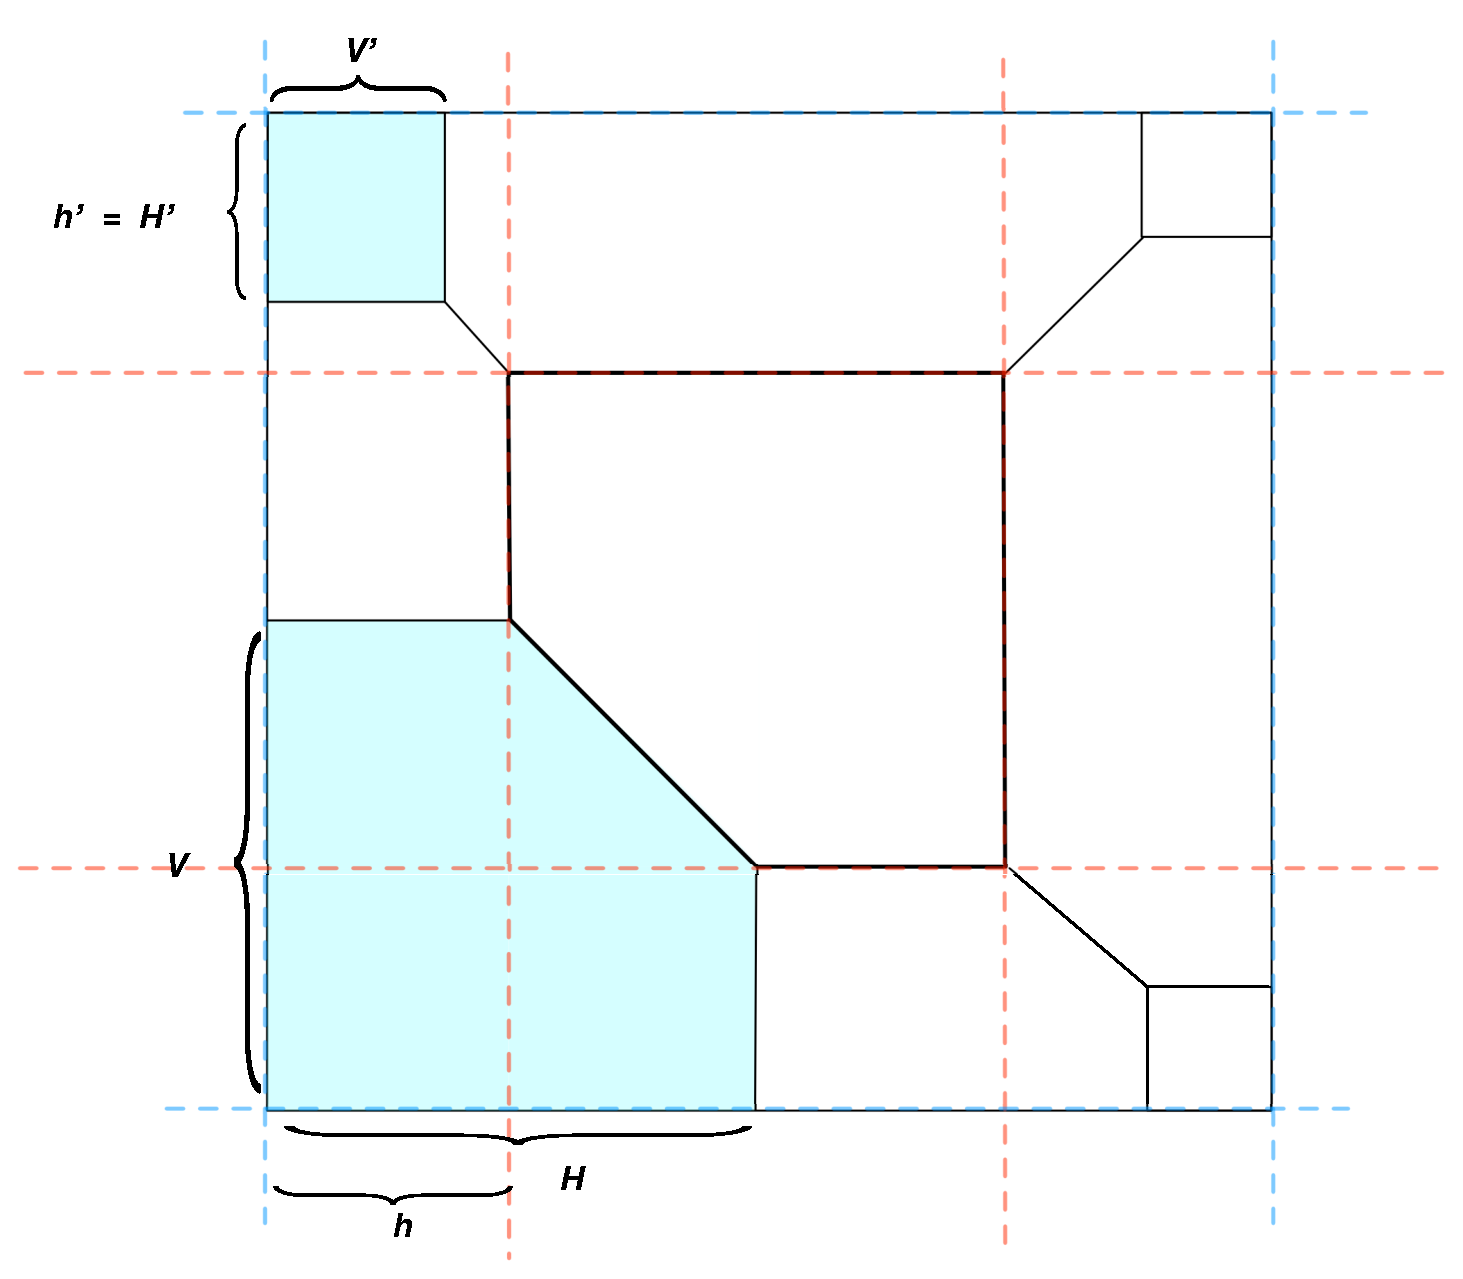
\includegraphics[width=0.8\textwidth]{minimal_tiles.eps}
    \caption{Illustration of fundamental dimensions to define each region's boundary: $h,H,V$ and
    $h',H',V'$.  We'll show in this section how to derive both bounds from the same function}\label{subfig:mintile}
  \end{subfigure}
  ~
  \begin{subfigure}[ht]{.4\textwidth}
    \centering
    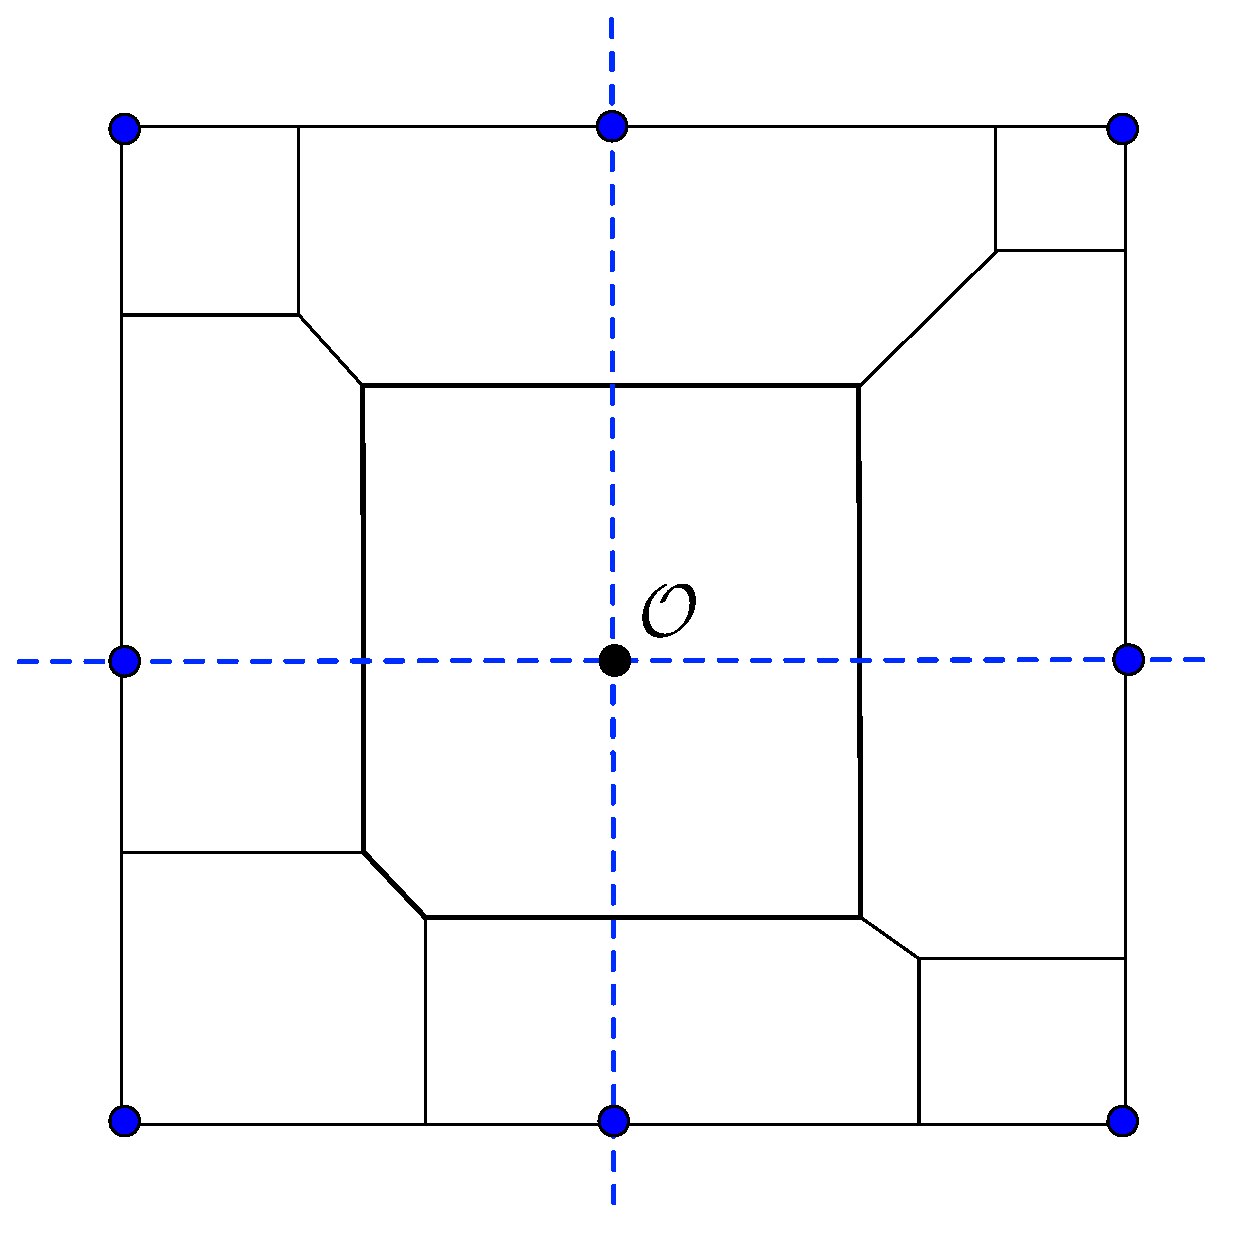
\includegraphics[width=\textwidth]{subdivision.eps}
    \caption{A subdivision of all regions by drawing a horizontal and vertical line through the origin
    $\mathcal{O}$ - note how each region now looks very similar to the regions annotated in \ref{subfig:mintile}}
    \label{subfig:subdivision}
    \end{subfigure}
  %\includegraphics[width=0.4\textwidth]{region_map.pdf}
  \caption{An illustration of the minimal set of dimensions needed for each region to be described by the same
  bounds.}
  \label{fig:tiles}
\end{figure}

\begin{algorithm}[h]
  \setcounter{AlgoLine}{0}
  \For{$\textsf{tile} \in \{\text{The tiles found in region }\;a_xa_y\}$}{\label{ln:all_tiles}
    \For{$i_x \la 1$ \KwTo $H(\textsf{tile})$}{ \label{ln:H}
      \For{$i_y \la 1$ \KwTo $\text{\bf min}( V(\textsf{tile}),V(\textsf{tile}) - i_x + h(\textsf{tile}) )$}{
        \label{ln:V}
        $\text{{\it Update the value at grid cell} $(i_x,i_y)$ {\it 1 timestep}}$\;
      }
    }
  }
  \caption{Procedure to update each region $a_xa_y$ according to the number of unit tiles present}
  \label{alg:tile_update}
\end{algorithm}


While the 9 regions above do not share the same dependency structure with respect to neighbor process cells,
they do share the same geometric forms which are captured by the corner regions: The pentagon of region
$-1-1$ and the squares of regions $1^-1$, $11$, and $^-11$ in figure~\ref{subfig:mintile} for example.
  The figure further illustrates dimensions
$H,h$ and $V$ for regions $-1-1$ and $^-11$ which capture both the pentagon and square shapes.
Therefore, to update any
region's grid cells, we can consider an approach outlined in the pseudocode
of algorithm~\ref{alg:tile_update}.
  In line~\ref{ln:all_tiles} of the pseudo code, we assume that the unit tiles
 illustrated in figure~\ref{subfig:mintile} can be derived as a function of
 the region $a_xa_y$, and then in lines \ref{ln:H}--\ref{ln:V} each dimension
 ($H,h$, and $V$) can
 be derived as a function of the region tiles.  This is a
 very rough outline of
 what we develop formally below, but it serves as a good guide for our
 intuition.

To further understand how each region provides the information needed to
determine the set of uniform tiles, consider figure~\ref{subfig:subdivision}.
This figure rescales figure~\ref{subfig:mintile} slightly and draws
a subdivion of each region
by intersecting perpendicular lines through an origin term (black center dot)
given by,
\begin{equation}
  \mathcal{O} \equiv \bigl[x_{^-1} + \frac{x_1 - x_{^-1}}{2}, \;\;\; y_{^-1} + \frac{y_1 - y_{^-1}}{2} \bigl].
  \label{eq:O}
\end{equation}
The intersecting lines through this point, cut accross the center of $00$ horizontally and vertically,
and cut acrross the other side regions
($01$,$0-1$,$10$,$-10$) either horizontally or vertically.  The highlighted blue dots then represent the
origins of each unit geometry which can be specified by $H$, $h$, and $V$ as illustrated
in figure~\ref{subfig:mintile}.

With this in mind, as long as we can concisely shift our origin and bounds for each region, we can use the
uniform iterates provided by algorithm~\ref{alg:tile_update} for every region and region subdivision.
We can do this via simple coordinate transformations,
and rotations.  Transformations are defined by
\begin{eqnarray}
  T_x(a_xa_y) &= B_x^1 \cdot \mathbf{max}(a_x,0) + (1 - |a_x|) \cdot \mathcal{O}_x\\
  T_y(a_xa_y) &= B_y^1 \cdot \mathbf{max}(a_y,0) + (1 - |a_y|) \cdot \mathcal{O}_y,
  \label{eq:transforms}
\end{eqnarray}
where $\mathcal{O}_x$ is the first term of definition \ref{eq:O}, and $\mathcal{O}_y$ the second term.  To
rotate our orientation in each region so that each region may share the same origin, we can employ the
standard rotation matrix in 2 dimensions,
\begin{equation}
  R_{\theta} \equiv \begin{bmatrix}
    \text{cos} (\theta) & - \text{sin}(\theta) \\
    \text{sin}(\theta) & \text{cos}(\theta)
    \end{bmatrix}.
\end{equation}

\begin{figure}[h]
  \centering
  \begin{subfigure}[h]{.5\textwidth}
    \centering
    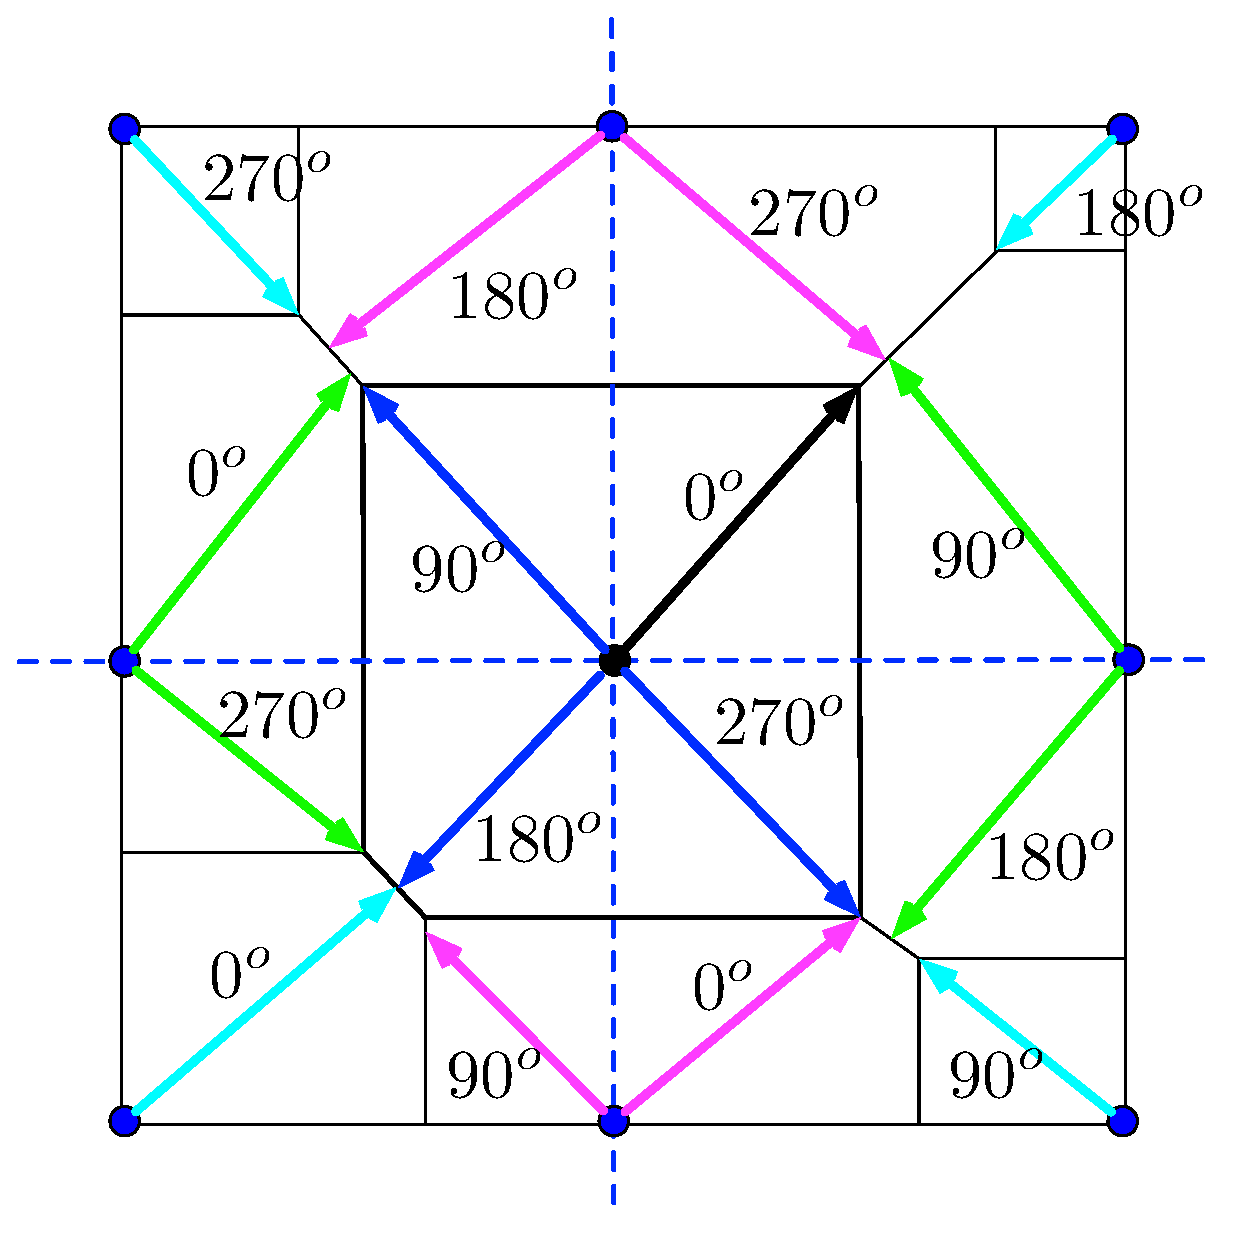
\includegraphics[width=.8\textwidth]{vectors.eps}
    \caption{Vectors and angles corrsponding to each
    region, with color coded sets of $0^o - 270^o$.  The
    angle is calculated relative to the unit vector of
    figure~\ref{subfig:unit}}
    \label{subfig:all_vectors}
  \end{subfigure}
  ~
  \begin{subfigure}[h]{.4\textwidth}
    \centering
    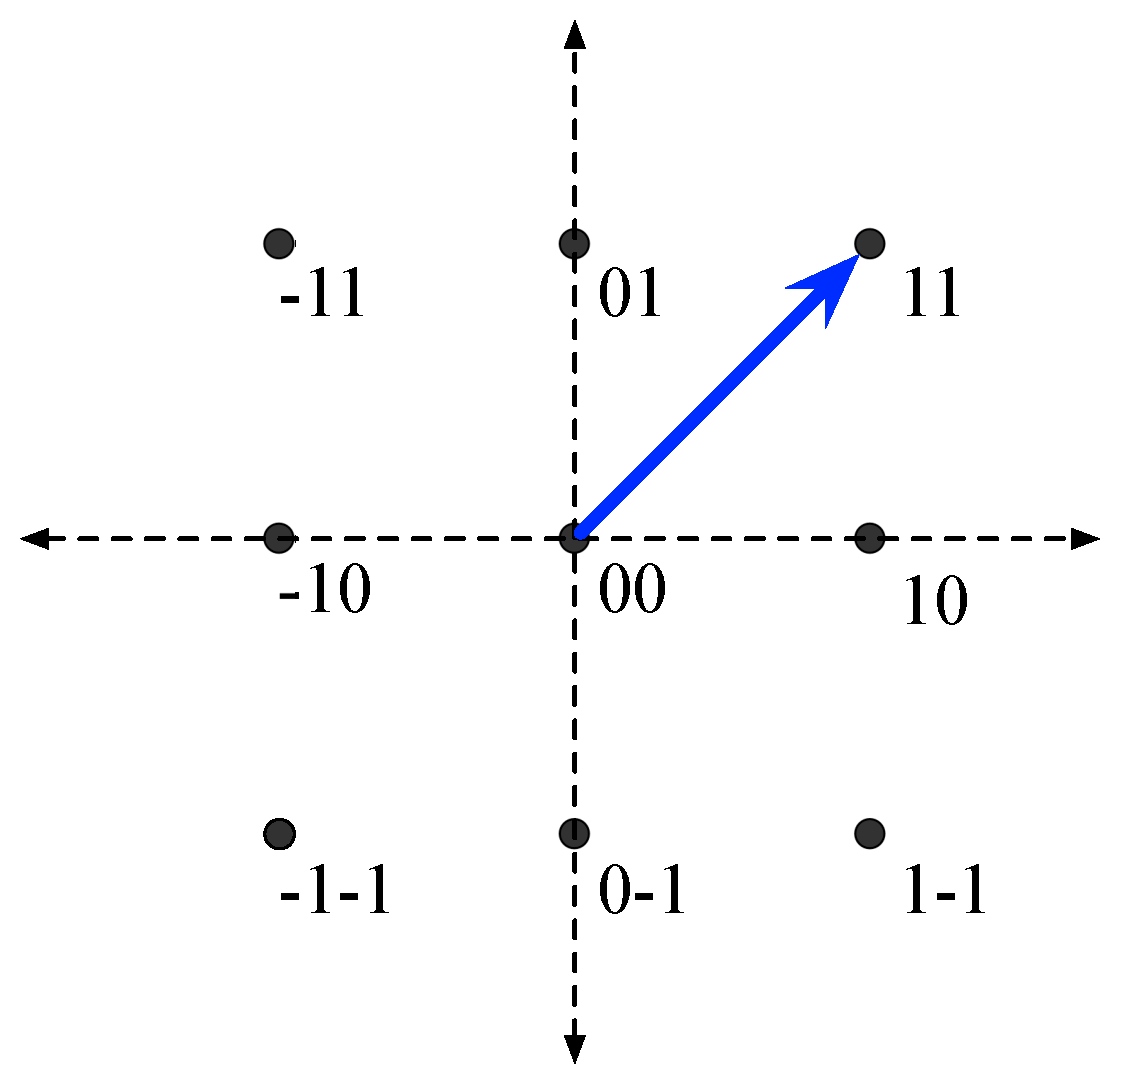
\includegraphics[width=\textwidth]{unit_square.eps}
    \caption{Unit vector overalayed on coordinates
    corresponding to region labels}
    \label{subfig:unit}
    \end{subfigure}
  %\includegraphics[width=0.4\textwidth]{region_map.pdf}
  \caption{Region angles, and the unit vector}
  \label{fig:vectors}
\end{figure}

To employ rotations properly, we'll need to know what rotations must be performed
in each region, for each subdivision.
Figure~\ref{subfig:all_vectors} illustrates the number of rotations present in each
region, along
with their rotation angles and the vectors they're derived from.  In practice, we'll
want a procedure to
derive these angles using only the region vector, $a_xa_y$.  To do so, it's necessary
to understand how
all of the vectors drawn in figure~\ref{subfig:all_vectors} acquire their angle and
magnitude.
Figure~\ref{subfig:unit} explains this in part by
illustrating the labels of each
region overlaid on a
cartesian plain, where the labels assemble to form a unit square centered on
$[0, \;\; 0]$.
Further, the unit vector whose
tail to head goes from $[0, \;\; 0]$ to $[1, \;\; 1]$ provides an orientation from
which to measure the angles in figure~\ref{subfig:all_vectors}.
  The vector of figure~\ref{subfig:unit} will be
  called the {\it unit vector}.  Our procedure for uncovering angles
for each region can now proceed as follows:
\begin{enumerate}
  \item Find the vectors which map to our unit tiles
  \item Find the angle between each vector and the unit vector
  \item return the set of angles.
\end{enumerate}
Given that we know the angles we're looking for--enumerated in figure~\ref{subfig:all_vectors}--
it is straightforward to verify the derived procedure.

\begin{algorithm}[hb]
  \setcounter{AlgoLine}{0}
  \Procedure{$AngleSearch(a_xa_y \in \mathcal{R})$}{
    $\mathcal{S}' = \{\}$\;

    \For{$s \in \mathcal{S}_u $}{
      $\mathcal{S}' = \mathcal{S}' \cup \{ \mathbf{s} + [a_x,\;\; a_y]\}$ \label{ln:as3}
    }
    $\mathcal{S}' = \mathcal{S}' \cap \mathcal{R}$\;  \label{ln:as4}

    $\Theta = \{\}$\;

    \For{$s \in \mathcal{S}' $}{
      $\mathbf{u} = \mathbf{s} - [a_x,\;\; a_y]$\;  \label{ln:as7}

      $\Theta = \Theta \cup atan2(\mathbf{u}\cdot\mathbf{v}^u, |\mathbf{u}^T || {\mathbf{v}^u}^T| )$\;  \label{ln:as8}
    }
    $\mathbf{return}\;\; \Theta$\;
  }
  \caption{Procedure, {\it AngleSearch} which takes as input $a_xa_y \in \mathcal{R}$,
  and returns the set $\Theta$ of all the angles associated with it.}
  \label{alg:angle_search}
\end{algorithm}

To find the angles enumerated in figure~\ref{subfig:all_vectors},
we formalize some notions of our unit labelings of each region:
\begin{flalign}
  \mathcal{R} \equiv &\;\; \{ -1-1,0-1,1-1,-10,00,10,-11,01,11 \}\\
  \mathcal{S}_u \equiv &\;\; \{ -1-1,1-1,-11,11 \}\\
  \mathbf{v}^u \equiv &\;\; [1, \;\; 1].
\end{flalign}
$\mathcal{R}$ is just the set of all possible regions given our breakdown where $a_xa_y \in \mathcal{R}$
always.  Note further that our notation for $a_xa_y$, can also be thought of as indicating a
vector $[a_x, \;\; a_y]$, and we will use the notations interchangably. $\mathcal{S}_u$ is a subset
of $\mathcal{R}$, and provides a way to derive the angles of figure~\ref{subfig:all_vectors}
along with the unit vector, $\mathbf{v}^u$.

Algorithm~\ref{alg:angle_search} formalizes the procedure outlined in steps
1-3 above, and proceeds as follows.  Line~\ref{ln:as3} adds every region vector
 $a_xa_y$ to each element of $\mathcal{S}_u$, before finding the intersection of these vectors with the set
 of valid labels in line~\ref{ln:as4}.  With these valid label's in hand, line~\ref{ln:as7} calculates the
  corresponding vectors of each region $a_xa_y$--
  in fact the $\mathbf{u}$ calculated here are the vectors
 displayed and color coded for each region in figure~\ref{subfig:all_vectors}.  Finally, the angle between
 the vector $\mathbf{u}$ and the unit vector $\mathbf{v}^u$ are calculated in
 line~\ref{ln:as7}.  The trigonometric function $atan2$ is used in order to return an angle between $0$ and
 $360$ to conform to our target rotations (figure~\ref{subfig:all_vectors}).  The inputs to this function
are the dot product of $\mathbf{u}$ and $\mathbf{v}^u$ followed by the determinant of the same vectors
concatenated together--concatenation denoted by $||$, and the determinant denoted with vertical bars on
each side of the expression, $| \cdot |$.

With our state composition defined in section~\ref{sec:state}, and our ability to isolate uniform tiles by
angle with
procedure~\ref{alg:angle_search}, we're now able to derive an expression for $H$, $h$, and $V$ illustrated in
figure~\ref{subfig:mintile}, and therefore  implement our update pseudocode outlined by
procedure~\ref{alg:tile_update}.  Specifically, each tile's dimensions ($H$, $h$, and $V$) can be
expressed as functions where $h,H,V: (a_xa_y,\theta) \ra \mathbb{R}^+$.
To develop these functions, we'll need a way to index state variables presented in section~\ref{sec:state}.
  The first observation that can aid intuition of the indexing scheme derived is to observe the core
  variables of state~\ref{eq:P} and~\ref{eq:D},
\[
  \mathbf{P} \equiv \begin{bmatrix}
    [x_{^-1}, y_{^-1}] & [x_1, y_{^-1}] \\
    [x_{^-1}, y_1] & [x_1, y_1]
  \end{bmatrix},
\]
and
\[
  \mathbf{\Delta} \equiv \begin{bmatrix}
    \delta_{^-1^-1} & \delta_{1^-1} \\
    \delta_{^-11} & \delta_{11}
    \end{bmatrix}.
\]

Note that for region $00$, $H,V$, and $h$ can all be written in terms of each term in these matrices
for each angle $\theta$ by moving counter-clockwise through the matrix~\ref{eq:P} starting
in the bottom right corner of each matrix (i.e. $\mathbf{P}_{11}$ and $\mathbf{\Delta}_{11}$).  For example
at $\theta=0^o$ for region $00$, $H,V$, and $h$ will all be bounded by $[x_1,\; y_1]$ and $\delta_{11}$
(i.e. the terms of $\mathbf{P}_{11}$ and $\mathbf{\Delta}_{11}$).  This observation on the pattern of
matrix indexing according to angle rotations can be generalized for rows (denoted \textsf{r}) and columns
(denoted \textsf{c}) of matrices as
\begin{flalign}
  \textsf{c} &= \mathbf{min}(1 + [R_{-\theta} \cdot \mathbf{v}^u]_y, 1)\\
  \textsf{r} &= \mathbf{min}(1 + [R_{-\theta} \cdot \mathbf{v}^u]_x, 1).
\end{flalign}
To simplify notation however, for any 2x2 matrix $M$ and
angle $\theta \in \{0,90,180,360\}$, we write
\begin{equation}
   M[\theta] \equiv M_{\textsf{rc}},
   \label{eq:tidx}
\end{equation}
Which allows us to directly index variables of state by angle $\theta$.  To do this for any region
$a_xa_y$ however, the expressions of state in their current matrix form would not be sufficient to
employ this kind of angle based indexing universally without first transforming the matrices of state
given by matrices~\eqref{eq:B}--\eqref{eq:D}.
This transformation is given by the following function, where for state matrix $M$,
region transformation $M_{a_xa_y}$, is defined as:
\begin{equation}
  M_{a_xa_y} \equiv \begin{pmatrix}
  0 & 1\\
  1 & 0
  \end{pmatrix}^{2-|a_y|} \cdot M \cdot \begin{pmatrix}
  0 & 1\\
  1 & 0
  \end{pmatrix}^{2-|a_x|},
  \label{eq:flips}
\end{equation}
where the pre-multiplication of matrix
$\begin{pmatrix}
  0 & 1\\
  1 & 0
  \end{pmatrix}$ flips the rows of matrix $M$, and the post-multiplication
of matrix $M$ by $\begin{pmatrix}
  0 & 1\\
  1 & 0
  \end{pmatrix}$ flips its columns.  Given our relatively small state space,
this can be verified as yielding appropriate matrices of state
for each region through an exhaustion of cases.

Taken together, equations~\ref{eq:tidx} and~\ref{eq:flips}, allow us to retrieve the variables
 of state given $\theta$ and $a_xa_y$,
\begin{eqnarray}
    \pv &= \mathbf{P}_{a_xa_y}[\theta] \label{eq:pv} \\
    \bv &= \mathbf{B}_{a_xa_y}[\theta]\\
    \delta &= \mathbf{\Delta}_{a_xa_y}[\theta]\\
    \uv &= \mathbf{U}_{a_xa_y}[\theta]. \label{eq:uv}
\end{eqnarray}
From equations~\ref{eq:pv}--~\ref{eq:uv}, we can write $h,H,V: (a_xa_y,\theta) \ra \mathbb{R}^+$,
\begin{equation}
    h(\theta,\av) = [\rnt \cdot \pv^T]_x + [\rnt \cdot \av^T]_x \cdot [\rnt \cdot \bv^T]_x -
    [\rnt \cdot \orig]_x \cdot (1 - |\rnt \cdot \av^T|_x) +
    (1 - |\rnt \cdot \av^T|_y) \cdot \mathbf{min}_{x,y}(\rnt \cdot \uv ) \cdot \delta
    \label{eq:h}
\end{equation}
\begin{equation}
    H(\theta,\av) = [\rnt \cdot \pv^T]_x + [\rnt \cdot \av^T]_x \cdot [\rnt \cdot \bv^T]_x -
    [\rnt \cdot \orig]_x \cdot (1 - |\rnt \cdot \av^T|_x) +
    |\rnt \cdot \av^T|_y \cdot [\rnt \cdot \uv ]_x \cdot \delta
    \label{eq:H}
\end{equation}
\begin{equation}
    V(\theta,\av) = [\rnt \cdot \pv^T]_y + [\rnt \cdot \av^T]_y \cdot [\rnt \cdot \bv^T]_y -
    [\rnt \cdot \orig]_y \cdot (1 - |\rnt \cdot \av^T|_y) +
    |\rnt \cdot \av^T|_x \cdot [\rnt \cdot \uv ]_y \cdot \delta
    \label{eq:V}
\end{equation}
Making these functions discrete (i.e. $h,H,V: (a_xa_y,\theta) \ra \mathbb{Z}^+$)
requires reworking equation~\ref{eq:O} with the ceiling function,
\begin{equation}
    \mathcal{O} \equiv \bigl[x_{^-1} + \ceil[\Big]{\frac{x_1 - x_{^-1}}{2}}, \;\;\;
                             y_{^-1} + \ceil[\Big]{\frac{y_1 - y_{^-1}}{2}} \bigl],
    \label{eq:discreteO}
\end{equation}
and using using it in equations~\eqref{eq:h}--\eqref{eq:V}.  Algorithm \ref{alg:updates}
puts these equations together and gives precise analytic form to
the pseudocode developed in algorithm~\ref{alg:tile_update}.

% TODO: DELETE
% \footnote{
%   Here's where the matrix notation developed gets abused.  Because we're looking at a matrix of vectors in some cases
%   ($\mathbf{P}$ above for example), operations~\ref{eq:flips} must act separately on the vector components, where
%   $\mathbf{P}^x = \begin{bmatrix}
%     x_{^-1} & x_1 \\
%     x_{^-1} & x_1
%   \end{bmatrix}$ and $\mathbf{P}^y = \begin{bmatrix}
%     y_{^-1} & y_{^-1} \\
%     y_1 & y_1
%   \end{bmatrix}$, and $\mathbf{P}_{a_xa_y}$ is actually computing $\mathbf{P}^x_{a_xa_y}$ and $\mathbf{P}^y_{a_xa_y}$
%   before rejoining. Likewise, operation~\ref{eq:tidx} is applied to the individual components of each matrix of vectors
%   before being rejoined again.  Tensor algebra may be able to simplify this slight of hand, but those formalisms are
%   still being researched.
% }

\begin{algorithm}[h]
  \setcounter{AlgoLine}{0}
  $\Theta = AngleSearch(a_xa_y)$\; \label{ln:as}
  \For{$\theta \in \Theta $}{
    \For{$j=0$ \KwTo $j=H(\theta, \av)$}{
      \For{$k=0$ \KwTo $k=\mathbf{min}\{V(\theta,\av), V(\theta,\av) - j + h(\theta, \av)$}{
        $\mathbf{i} = \rt \cdot [j, \;\; k]^T$\;
        $g(t,T_x(\av) + \mathbf{i}_x
        T_y(\av) + \mathbf{i}_y)) =
        f(t-1,T_x(\av) + \mathbf{i}_x,
        T_y(\av) + \mathbf{i}_y)$
        \label{ln:update}
      }
    }
  }

  \caption{Uniform Region Update $\forall \text{ input } a_xa_y = \av \in \mathcal{R}$}
  \label{alg:updates}
\end{algorithm}

Algorithm~\ref{alg:updates} puts everything together ignoring some implemtation details,
with equations for $H,h,$ and $V$.
In the interest of concision, line~\ref{ln:update} omits a precise definition of a 5
point stencil, but simply states that $g(t,x,y) = f(t,x,y)$ meaning at time
$t$, we can compute the value of a stencil at $g(t,x,y)$ given some function $f$
of the same point $x,y$ at the prior time $t-1$.
Line~\ref{ln:as} executes the procedure of algorithm~\ref{alg:angle_search},
and illustrates the parallel between our notion of a tile and
it's apparent encoding as an angle.  The potential for
an intersection in the mathematical research on {\it tiling} is
intriguing, but has yet to bear analytic fruit beyond the broad
observations made in this section.


% % TODO: Possibly delete:
% % With these formalisms we can also rewrite algorithm~\ref{alg:state_updates_basic}
% % in a slightly more compact form as algorithm~\ref{alg:state_updates_compact}.

% % NOTE This seems to work, but is more compact
% %      and illicits less understanding
% % \begin{algorithm}[h]
% %   \setcounter{AlgoLine}{0}
% %   $\Theta = \text{AngleSearch}(a_xa_y)$\;
% %   $x_{^{^-}1} = x_{^{^-}1} + (1-|a_x|\cdot|ay|)\cdot ( 1-2\cdot\textsf{max}(|a_x|,|a_y|))$\;
% %   $y_{^{^-}1} = y_{^{^-}1} + (1-|a_x|\cdot|ay|)\cdot ( 1-2\cdot\textsf{max}(|a_x|,|a_y|))$\;
% %   $x_{1} = x_{1} + (1-|a_x|\cdot|ay|)\cdot ( 2\cdot\textsf{max}(|a_x|,|a_y|) -1) $\;
% %   $y_{1} = y_{1} + (1-|a_x|\cdot|ay|)\cdot ( 2\cdot\textsf{max}(|a_x|,|a_y|) -1) $\;
% %   $\Delta' = \Delta_{a_xa_y}$\;
% %   \For{$\theta \in \Theta$}{
% %     $\Delta'[\theta] = \Delta[\theta] +
% %     2\cdot\textsf{max}(|a_x|\cdot|a_y|,(1-|a_x|)\cdot(1-|a_x|)) - 1$
% %   }
% %   \caption{Procedure to update state values for each region $a_xa_y$}
% %   \label{alg:state_updates_compact}
% % \end{algorithm}


\section{Update Constraints for the Multi-Process Problem}

Up until now we've been considering updates on a single process using the regions decomposed by the state
laid out in section~\ref{sec:state}, but we still need to consider coordination between processes.
Recall in our discussion of algorithm~\ref{alg:state_updates_basic} that if the procedure is called
once for every region (i.e. $\forall a_xa_y \in \mathcal{R}$), then the borders introduced in the static
region decomposition in section~\ref{sec:problem_statement} remain unchanged.  However when this requirement
is relaxed, then a few things immediately follow.  In
particular, certain conditions must be met for algorithm~\ref{alg:updates} to be invoked by a process at all.  This
section enumerates those conditions.

\subsection{Nonzero Region Area}

This first such condition is that for every region $a_xa_y \in \mathcal{R}$, and for all
$\theta\in AngleSearch(a_xa_y)$, it must be the case that $h(\theta,a_xa_y) > 0$,
$H(\theta,a_xa_y) > 0$, and $V(\theta,a_xa_y) > 0$.  This can be summarized by the
boolean function,
\begin{equation}
    \mathcal{G}^S(a_xa_y,\Theta) \equiv \underset{\theta \in \Theta}{\wedge}
    H(\theta,\mathbf{a}) > 2 \wedge
    h(\theta,\mathbf{a}) > 2 \wedge
    V(\theta,\mathbf{a}) > 2,
    \label{eq:space_guard}
\end{equation}
where $\Theta = AngleSearch(a_xa_y)$.
Here, $0$ is replaced by $2$ given that in discrete space, a 5 point stencil must have at
minimum a $3x3$ grid of cells to update a single point
(or at least 5 cells, with its 4 corners missing).  We'll refer to formula~\ref{eq:space_guard}
as the {\it spatial update guard}.

\subsection{Interprocess Communication Constraints}

Any process wishing to update its border cells must receive ghost
cells from one or more neighbor processes.
Therefore, there must be a means of ensuring that the requisite
{\it communication} (sending and receiving of data) is performed
and completed.
Given our assumption that communication completion is nondeterministic, the abstraction
we will use will mimic MPI's non-blocking communication.  Let
every process have a unique id $\pid \in \mathbb{Z}^+$.  Let
the $\mathcal{N}(a_xa_y,\pid): (a_xa_y,\pid) \ra \{\mathbb{Z}^+\}$ be a mapping
from a region $a_xa_y$ and a process id $\pid$ to a set of positive
integers which themselves are process ids of the processes that
$\pid$ must communicate with (these ids are referred to as {\it neighbors}).

Next, we define functions analagous to MPI's
$\textsf{\textup{ISend}}$ and $\textsf{\textup{IRecv}}$ respectively.
$\textsf{send}_{a_xa_y}[n] \la \psendf(n\in\mathbb{Z}^+,\textsf{d})$ is the signature for
a function which takes a neighbor process id as its first argument, and some
arbitrary data structure $\textsf{d}$ as its second argument, and returns a boolean value
in the array $\textsf{send}_{a_xa_y}[0..|\mathcal{N}(a_xa_y,\pid)|]$,
 which is initially set to false, and then
nondeterministically set to true when the neighbor process $n$ receives
the value $\textsf{d}$, and copies it to a local data structure.  Likewise,
$\textsf{rcv}_{a_xa_y}[n] \la \precvf(n\in\mathbb{Z}^+,\textsf{d})$ is the signature for
a function which takes a neighbor process id as its first argument, and some
arbitrary local data structure $\textsf{d}$ as its second argument,
and returns a boolean value
in the array $\textsf{rcv}_{a_xa_y}[0..|\mathcal{N}(a_xa_y,\pid)|]$,
 which is initially set to false, and then
nondeterministically set to true when the neighbor process
$\pid$ receives a new value in its local data structure $\textsf{d}$
from process $n$, and can perform a validly access the memory for $\textsf{d}$.

Given these definitions for communication between neighbor processes, it follows
for all $a_xa_y\in\mathcal{R} - \{00\}$ that the following boolean function
must be true for any valid update to be performed:
\begin{equation}
    \mathcal{G}^C(a_xa_y,\pid) \equiv \underset{n \in \mathcal{N}(a_xa_y,\pid)}{\wedge}
    \textsf{send}_{a_xa_y}[n] \wedge \textsf{rcv}_{a_xa_y}[n].
    \label{eq:comm_guard}
\end{equation}
We'll call this the {\it communication update guard}.

\subsection{Mirror Process Misalignment}

\begin{figure}[h]
    \centering
    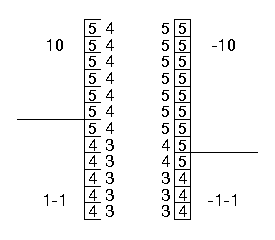
\includegraphics[width=.3\textwidth]{mirrorPaperFinal.eps}
    \caption{A motivating example for the utility of $\mathcal{G_M}$.  A subset of the
    2D data arrays of a left and right process are illustrated--ghost cells drawn without a border, and
    border cells given a border.  A delimeter between regions on each process perpendicular To
     $B_x^{1}$ and $B_x^{^-1}$ is drawn for the left and right process, respectively.  Region labels
     are shown for the 4 regions of interest to the example, and the rest are omitted}
    \label{fig:mirror_motivation}
\end{figure}

Given a global spatial decomposition as described in section~\ref{sec:problem_statement},
2 neighbor processes are referred to as
{\it mirror processes} of each other.  In figure~\ref{fig:basic}, process 2 and 4 are process 1's mirror
processes, process 1 and 3 are process 2's mirror processes, and so on.  Further,
the state variables outlined in section~\ref{sec:state} are referred to as the
{\it mirror state} of the processes adjacent to them.

Figure~\ref{fig:mirror_motivation} illustrates an example how the {\it mirror state}
of 2 processes can become misaligned.  This discussion will not show how such a state
is reachable, but what must be done when it occurs in order to respect the dependency
contraints of a cell update at the border.
Drawn is a left process with regions $-10$ and $10$ shown,
and its {\it mirror process} on the right with regions $-10$ and $-1-1$.  Border cells
of the processes are bordered by a square boxes, and a timesteps are displayed within them.
Ghost cell timesteps are displayed with no border.
\begin{algorithm}[h]
  % NOTE: Mirror state has the same matrix flips as the the current state, so at least for
  % the actual implementation of things, this would need to be accounted for
  \setcounter{AlgoLine}{0}
  \Procedure{$\mathcal{G}^M(a_xa_y \in \mathcal{R}-\{00\}, \Theta)$}{
    % \When{$a_xa_y = 00$}{
    %     $\mathbf{return}\;\;\;  \textsf{true}$\;
    % }
    $\theta_1 = \Theta[0]$; $\;\;\;\theta_2 = \Theta[1] \;\mathbf{ ? }\; |\Theta| = 2 \;\mathbf{ : }\; \theta_1$\;
    $\mathbf{return }\;\; H[\theta_1] \leq V^M[\theta_1 - 90] \wedge
    V[\theta_2] \leq V^M[\theta_2 + 90] $\;
  }
  \caption{Procedure to check mirror state for each
  $a_xa_y \in \mathcal{R}$}
  \label{alg:mirror_guard}
\end{algorithm}
Observe that the border cells
of the left process are exactly reflected in the ghost cells of the right process and
vice~versa.  This in fact corresponds to the state in each process, $\mathbf{P}$ and
$\mathbf{\Delta}$.  We assume further that this state is exchnaged between processes,
and stored as locally in {\it mirror variables}, where
\begin{eqnarray}
  \mathbf{\Delta}_n^M &\equiv \mathbf{\Delta}\;\text{matrix of neighbor process $n$}\\
  \mathbf{P}_n^M &\equiv \mathbf{P}\;\text{matrix of neighbor process $n$}.
\end{eqnarray}
It follows, that any calculation made with these terms will receive a superscript $M$
to denote that it is in fact measuring the term for the mirror process (e.g.
$V^M(\theta, \mathbf{a}), h^M(\theta, \mathbf{a})$).

To ensure that
a region $a_xa_y$ is not updated when its appropriate ghost cells are not present
as in region $-10$ in figure~\ref{fig:mirror_motivation}, the boolean function
$\mathcal{G}^M$ shown in algorithm~\ref{alg:mirror_guard} can be used.  The function
returns $\textsf{true}$ if the region is an interior region, and then checks alignment
with mirror quantities from its neigbor process(es).  $H(\theta,\mathbf{a})$ is
mirrored by $V^M(\theta - 90^o,\mathbf{a})$, and $V(\theta,\mathbf{a})$ is mirrored
by $V^M(\theta + 90^o,\mathbf{a})$.  This is a relationship that holds up for all
$a_xa_y \in \mathcal{R} - \{00\}$, and can be checked by drawing out the rotated bounds
$V$ and $H$ for all border and corner regions, along side their region bounds.
% TODO: Double check, but this may not be necessary at all if we're overwriting
%       mirror state for each neighbor $n$.
% \begin{algorithm}[h]
%   % % %% TODO: If corner, need to assert that the latest timestep is strictly
%   % % %%       less than or equal to the middle regions
%   \setcounter{AlgoLine}{0}
%   \Procedure{$\mathcal{G}^T(a_xa_y \in \mathcal{R}, \Theta)$}{
%     \When{$a_xa_y = 00$}{
%         $\mathbf{return}\;\;\;  \textsf{true}$\;
%     }
%     $ready = \textsf{true}$\;
%     \For{$\theta \in \Theta $}{
%       $\mathbf{i} = \rt \cdot [H(\theta,\av), V(\theta,\av)]$\;
%       % TODO: Do we need to rotate these as well to get the signs right
%       $b = \rnt \cdot B_{a_xa_y}[\theta]$\;
%       $\dx = \textsf{sign}(\mathbf{i}_x)$;
%       $\;\;\dy = \textsf{sign}(\mathbf{i}_y)$\;
%       $ready \;\wedge= a_{x+\dx}a_y \in \mathcal{R} - \{00\} \wedge
%       t(a_xa_y, T_x + b_x + \mathbf{i}_x,
%       T_y + b_y) = t_{a_{x+\dx}a_y}^M(T_x + b_x + \mathbf{i}_x + \dx,
%       T_y + b_y)$\;

%       $ready \;\wedge= a_xa_{y+\dy} \in \mathcal{R} - \{00\} \wedge
%       t(a_xa_y, T_x + b_x,
%       T_y + b_y + \mathbf{i}_y) = t_{a_xa_{y+\dy}}^M(T_x + b_x,
%       T_y + b_y + \mathbf{i}_y + \dy)$\;
%     }
%     $\mathbf{return}\;\;\;  ready$\;
%   }
%   \caption{Guard routine to check that neighbors are aligned for
%   regions $a_xa_y \in \mathcal{R}$, named $\mathcal{G}^T$}
%   \label{alg:time_guard}
% \end{algorithm}

% Image~\ref{fig:mirror_motivation} also provides a clue for how to check
% whether or not the ghost cells are sufficiently updated for a border
% region to have all of its cell dependencies met.  Note that the ghost
% cells of $-10$ and $-1-1$ violate the function~\eqref{eq:ts} on the
% boundary of the 2 regions (there is a 'plateau' in the timestep rather
% than a strictly increasing step as described by equation \eqref{eq:ts}).

% Even if mirror state happens to be stale, algorithm \ref{alg:time_guard}
% can check whether or not this relationship is

\section{Full Algorithm}

\begin{algorithm}[h]
  \setcounter{AlgoLine}{0}
  \tcc{Initialize Global Variables.}
  $\tm\la 1$\;
  $x_{^-1}\la 1$; $x_1\la B_x^1$; $y_{^-1} \la 1$; $y_1 \la B_y^1$\;
  $\delta_{^-11}\la 0$; $\delta_{^-1^-1}\la 0$; $\delta_{11}\la 0$; $\delta_{1^-1}\la 0$\;


  \For{$a_xa_y \in \mathcal{R}-\{00\}$}{ % Initialize communication
      $\Theta = \text{AngleSearch}(a_xa_y)$\;
      \For{$\theta \in \Theta $}{
          \For{$n \in \mathcal{N}(a_xa_y,\pid)$}{
              $\textsf{send}_{a_xa_y}[n] \la \psend{n}{\mathbf{\Delta}}$;
              $\;\;\textsf{rcv}_{a_xa_y}[n] \la \precv{n}{\mathbf{\Delta}^M_n}$\;
              $\textsf{send}_{a_xa_y}[n] \la \psend{n}{\mathbf{P}}$;
              $\;\;\textsf{rcv}_{a_xa_y}[n] \la \precv{n}{\mathbf{P}^M_n}$\;
              $\textsf{send}_{a_xa_y}[n] \la \psend{n}{\data[1]
              [\mathbb{I}_y(-1, \theta,\mathbf{a})^s..\mathbb{I}_y(+1, \theta,\mathbf{a})^s]
              [\mathbb{I}_x(-1, \theta,\mathbf{a})^s..\mathbb{I}_x(+1, \theta,\mathbf{a})^s]}$;
              $\;\;\textsf{rcv}_{a_xa_y}[n] \la \precv{n}{\data[0]
              [\mathbb{I}_y(-1, \theta,\mathbf{a})..\mathbb{I}_y(+1, \theta,\mathbf{a})]
              [\mathbb{I}_x(-1, \theta,\mathbf{a})..\mathbb{I}_x(+1, \theta,\mathbf{a})]}$\;
          }
      }
  }
  % While loop for state (time and space)
  \While(){$\tm < \textsf{nsteps} \vee x_{^-1} > 0 \vee y_{^-1} > 0 \vee x_{1} < B_x^1 \vee y_{^-1} > B_y^1$}{
      \For{$a_xa_y \in \mathcal{R}$}{
          $\Theta = \text{AngleSearch}(a_xa_y)$\; \label{ln:fas}

          \When{$ \mathcal{G}^S(a_xa_y, \Theta) \wedge (
              (
                  \mathcal{G}^C(a_xa_y,\pid) \wedge
                  \mathcal{G}^M(a_xa_y, \Theta)
              ) \vee a_xa_y = 00
              )$}{
              $\theta_c = 0$\;
              \For{$\theta \in \Theta $}{
                  $\pv = \mathbf{P}_{a_xa_y}[\theta]$\;
                  $\bv = \mathbf{B}_{a_xa_y}[\theta]$\;
                  $\delta = \mathbf{\Delta}_{a_xa_y}[\theta]$\;
                  $\uv = \mathbf{U}_{a_xa_y}[\theta]$\;
                  $h(\theta,\av) = [\rnt \cdot \pv^T]_x + [\rnt \cdot \av^T]_x \cdot [\rnt \cdot \bv^T]_x -
                  [\rnt \cdot \orig]_x \cdot (1 - |\rnt \cdot \av^T|_x) +
                  (1 - |\rnt \cdot \av^T|_y) \cdot \mathbf{min}_{x,y}(\rnt \cdot \uv ) \cdot \delta$\;
                  $H(\theta,\av) = [\rnt \cdot \pv^T]_x + [\rnt \cdot \av^T]_x \cdot [\rnt \cdot \bv^T]_x -
                  [\rnt \cdot \orig]_x \cdot (1 - |\rnt \cdot \av^T|_x) +
                  |\rnt \cdot \av^T|_y \cdot [\rnt \cdot \uv ]_x \cdot \delta$\;
                  $V(\theta,\av) = [\rnt \cdot \pv^T]_y + [\rnt \cdot \av^T]_y \cdot [\rnt \cdot \bv^T]_y -
                  [\rnt \cdot \orig]_y \cdot (1 - |\rnt \cdot \av^T|_y) +
                  |\rnt \cdot \av^T|_x \cdot [\rnt \cdot \uv ]_y \cdot \delta$\;
                  $\mathbf{q} = \rt \cdot [1, \;\; 1]^T$\;
                  \For{$j=0$ \KwTo $j=H(\theta, \av) - \mathbf{q}_x$}{
                      \For{$k=0$ \KwTo $k=\mathbf{min}\{V(\theta,\av) - \mathbf{q}_y, V(\theta,\av) - j + h(\theta, \av) - \mathbf{q}_y\}$}{
                          $\mathbf{i} = \rt \cdot [j, \;\; k]^T$\;
                          $\data[1-\overline{t(a_xa_y,j,k)}]
                          [T_y(\av) + \mathbf{i}_y) + \mathbf{q}_y \cdot (1-|a_y|) \cdot \mathbf{min}((\theta_c \;\mathbf{mod}\; 3),1)]
                          [T_x(\av) + \mathbf{i}_x + \mathbf{q}_x \cdot (1-|a_x|) \cdot \overline{\theta_c}]
                          =
                          f'(\data[\overline{t(a_xa_y,j,k)}]
                          [T_y(\av) + \mathbf{i}_y + \mathbf{q}_y \cdot (1-|a_y|) \cdot \mathbf{min}((\theta_c \;\mathbf{mod}\; 3),1)]
                          [T_x(\av) + \mathbf{i}_x + \mathbf{q}_x \cdot (1-|a_x|) \cdot \overline{\theta_c}])$
                          \label{ln:fupdate}
                      }
                  }
                  $\theta_c = \theta_c + 1$\;
              }
              \When{$a_xa_y \neq 00$}{
                  \For{$\theta \in \Theta $}{
                      \For{$n \in \mathcal{N}(a_xa_y,\pid)$}{
                          $\textsf{send}_{a_xa_y}[n] \la \psend{n}{\mathbf{\Delta}}$;
                          $\;\;\textsf{rcv}_{a_xa_y}[n] \la \precv{n}{\mathbf{\Delta}^M_n}$\;
                          $\textsf{send}_{a_xa_y}[n] \la \psend{n}{\mathbf{P}}$;
                          $\;\;\textsf{rcv}_{a_xa_y}[n] \la \precv{n}{\mathbf{P}^M_n}$\;
                          $\textsf{send}_{a_xa_y}[n] \la \psend{n}{\data[1-\overline{t(a_xa_y,j,k)}]
                          [\mathbb{I}_y(-1, \theta,\mathbf{a})^s..\mathbb{I}_y(+1, \theta,\mathbf{a})^s]
                          [\mathbb{I}_x(-1, \theta,\mathbf{a})^s..\mathbb{I}_x(+1, \theta,\mathbf{a})^s]}$;
                          $\;\;\textsf{rcv}_{a_xa_y}[n] \la \precv{n}{\data[\overline{t(a_xa_y,j,k)}]
                          [\mathbb{I}_y(-1, \theta,\mathbf{a})..\mathbb{I}_y(+1, \theta,\mathbf{a})]
                          [\mathbb{I}_x(-1, \theta,\mathbf{a})..\mathbb{I}_x(+1, \theta,\mathbf{a})]}$\;
                      }
                  }
              }
              \When{$a_xa_y = 00$}{
                  $\tm \la \tm + 1$\;
              }
              $update\_state(a_xa_y)$\;
          }
      }
  }
  \caption{Full algorithm to be run on every process until termination conditions are met}
  \label{alg:full}
\end{algorithm}

The full description for a parallel decomposition of a 5 point stencil
is provided in algorithm \ref{alg:full}.  Some details that haven't been
explored are provided here for completeness.
To start with, how to handle discrete space indexing given rotations
within a region $a_xa_y$.  The modulo terms below account for this (where
$r = x \;\mathbf{mod}\; y$, and $r$ is the remainder from dividing
$x$ into $y$).  Given its frequency, the shorthand
 $\overline{x} = x \;\mathbf{mod}\; 2$ is used as well when $y=2$.
Additionally, a termination condition has not been introduced for the
algorithm.  Recall that the modeling problem initially set out in section
\ref{sec:problem_statement} is that of PDEs, which evolves a spatially dependent
quantity over time.  Therefore the stopping condition will be the number of
timesteps to evolve the spatial property over, $\textsf{nsteps}$.

Finally, we will actually introduce operations on an array of cells being used
to model the PDE.  $\data[0..1][0..B_y^1+1][0..B_x^1+1]$ will
hold all the grid cells regardless of region, including the ghost cells.  It
is a 3D array with a 'double buffering' strategy for updating in time
in the first dimension, and the height and length of the local portion
of the process' PDE stored in the rows and columns, respectively.  For
 a set of shorthands for defining the bounds to send and receive in
 each spatial dimension of $\data$ we define
\begin{eqnarray}
    \mathbb{I}_x(q, \theta,\mathbf{a}) &= T_x + |a_x|\cdot (a_x - q) \cdot \rt \cdot [H(\theta,\mathbf{a}),V(\theta,\mathbf{a})]^T_x\\
    \mathbb{I}_y(q, \theta,\mathbf{a}) &= T_y + |a_y|\cdot (a_y - q) \cdot \rt \cdot [H(\theta,\mathbf{a}),V(\theta,\mathbf{a})]^T_y,
\end{eqnarray}
where $q\in \{-1, 1\}$ indicating the left bound and right bound respectively.
This is a discrete function which works for the receive buffers (ghost cells), but given
we're also accessing send buffers (border cells), this won't be sufficient.
This combined with the need to account for the case where
$\mathbb{I}_x(-1,\theta,\mathbf{a}) = \mathbb{I}_x(+1,\theta,\mathbf{a})$ motivates
the additional helper function
\begin{eqnarray}
    \mathbb{I}_x(q,\theta,\mathbf{a})^s &= \textbf{min}(\textbf{max}(\mathbb{I}_x(q,\theta,\mathbf{a})-q,1),B_x^1)\\
    \mathbb{I}_y(q,\theta,\mathbf{a})^s &= \textbf{min}(\textbf{max}(\mathbb{I}_y(q,\theta,\mathbf{a})-q,1),B_y^1).
\end{eqnarray}
Finally, note that we do not define the entire stencil update
method for a 5 point stencil, but continue to denote it by
$f'$, which no longer needs a variable of time
(as in algorithm~\ref{alg:updates}), as our
$\data$ buffer has made this access precise.  Further,
$g$ has been dropped from the original formulation of
algorithm
\ref{alg:updates} as the left hand side of the update
need only access
the single appropriate center cell of the 5-point
dependency structure under study.